\begin{center}
    \textbf{Geração 100}
\end{center}

\begin{figure}[h]
    \centering
    \label{fig:geracaoXX}
    
    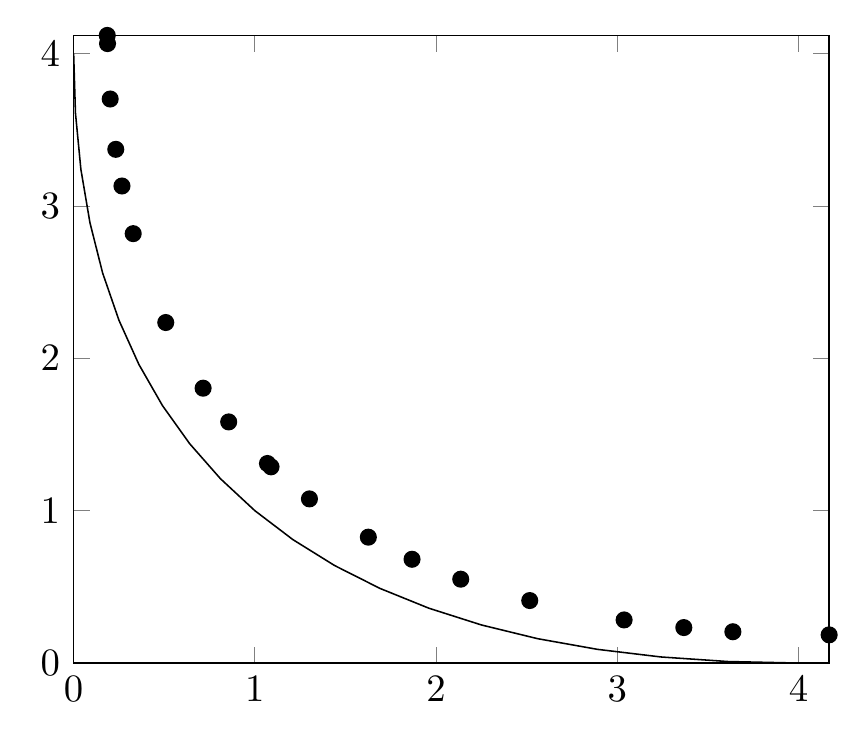
\begin{tikzpicture}[scale=1.4]
        \begin{axis}[enlargelimits=false]
            \addplot [] coordinates {
                (0.000000,4.000000) (0.010000,3.610000) (0.040000,3.240000) (0.090000,2.890000) (0.160000,2.560000) (0.250000,2.250000) (0.360000,1.960000) (0.490000,1.690000) (0.640000,1.440000) (0.810000,1.210000) (1.000000,1.000000) (1.210000,0.810000) (1.440000,0.640000) (1.690000,0.490000) (1.960000,0.360000) (2.250000,0.250000) (2.560000,0.160000) (2.890000,0.090000) (3.240000,0.040000) (3.610000,0.010000) (4.000000,0.000000) 
            };
            
            \addplot [only marks] coordinates {
                (4.168578,0.185014) (0.185481,4.119608) (0.508235,2.235170) (1.301067,1.077486) (0.714368,1.804074) (0.328600,2.818474) (1.625955,0.826308) (0.855511,1.582758) (1.069318,1.309841) (0.201713,3.702131) (2.516477,0.410313) (1.089113,1.288015) (3.037264,0.283012) (0.186988,4.065829) (0.232462,3.371838) (1.867110,0.681172) (3.366609,0.232987) (2.135822,0.550495) (3.637344,0.205522) (0.266636,3.131241) 
 
            };
        \end{axis}
    \end{tikzpicture}
\end{figure}